\documentclass{article}
\usepackage{graphicx}
\usepackage{listings}
\usepackage{xcolor}
\usepackage{amsmath}
\usepackage[a4paper, margin=1in]{geometry}
\setlength{\parindent}{0pt}

\title{Week6 Lab1 Report}
\author{111062117, Hsiang-Sheng Huang}

\begin{document}

\maketitle

\section*{HPL (High-Performance Linpack)}

\subsection*{Setting of N}

N is the matrix dimension used in HPL and is the number of rows and columns in the matrix. That is, the matrix is $N \times N$.

\vspace{1em}

N should be $80\% \sim 85\%$ of the total memory size, and there is a reference formula:

\begin{align*}
N = \sqrt{\frac{\texttt{Total\ Memory}}{8}}
\end{align*}

So first we use the following command to check the total memory size:

\begin{lstlisting}[language=bash, basicstyle=\ttfamily\small, numbers=left, numberstyle=\tiny\color{gray}, stepnumber=1, frame=single]
$ cat /proc/meminfo | grep MemTotal
\end{lstlisting}

The output is:

\begin{lstlisting}[language=bash, basicstyle=\ttfamily\small, numbers=left, numberstyle=\tiny\color{gray}, stepnumber=1, frame=single]
MemTotal:        3930592 kB
\end{lstlisting}

Then we can calculate the value of N:

\begin{align*}
\texttt{Total\ Memory} & = 3930592 \text{ kB} \\
N & = \sqrt{\frac{3930592 \times 1024}{8}} \\
    & \approx 22450
\end{align*}

This is the value of N assuming all memory is used to store the matrix.

\vspace{1em}

To avoid OOM (Out Of Memory), we set $80\% \sim 85\%$ of the total memory size.

\begin{itemize}
    \item $N = 22450 \times \sqrt{0.8} \approx 20070$
    \item $N = 22450 \times \sqrt{0.85} \approx 20700$
\end{itemize}

Also, we would like to set N to a multiple of NB, so we can set N to 20480.

\subsection*{Setting of NB}

NB is the block size used in HPL. The block size is the number of rows and columns in the sub-matrix. That is, the sub-matrix is $\text{NB} \times \text{NB}$.

\vspace{1em}

NB values in [32 ... 256] can achieve good performance.

\vspace{1em}

Here we set NB to 64.

\subsection*{Setting of P and Q}

P and Q are the number of processes in the row and column of the process grid. The product of P and Q should be equal to the number of processes used in HPL.

\vspace{1em}

The number of processes used in HPL is 8, so here we set $P = 2$ and $Q = 4$.

\subsection*{Results}

The following image shows the results.

\begin{figure}[htbp]
    \centering
    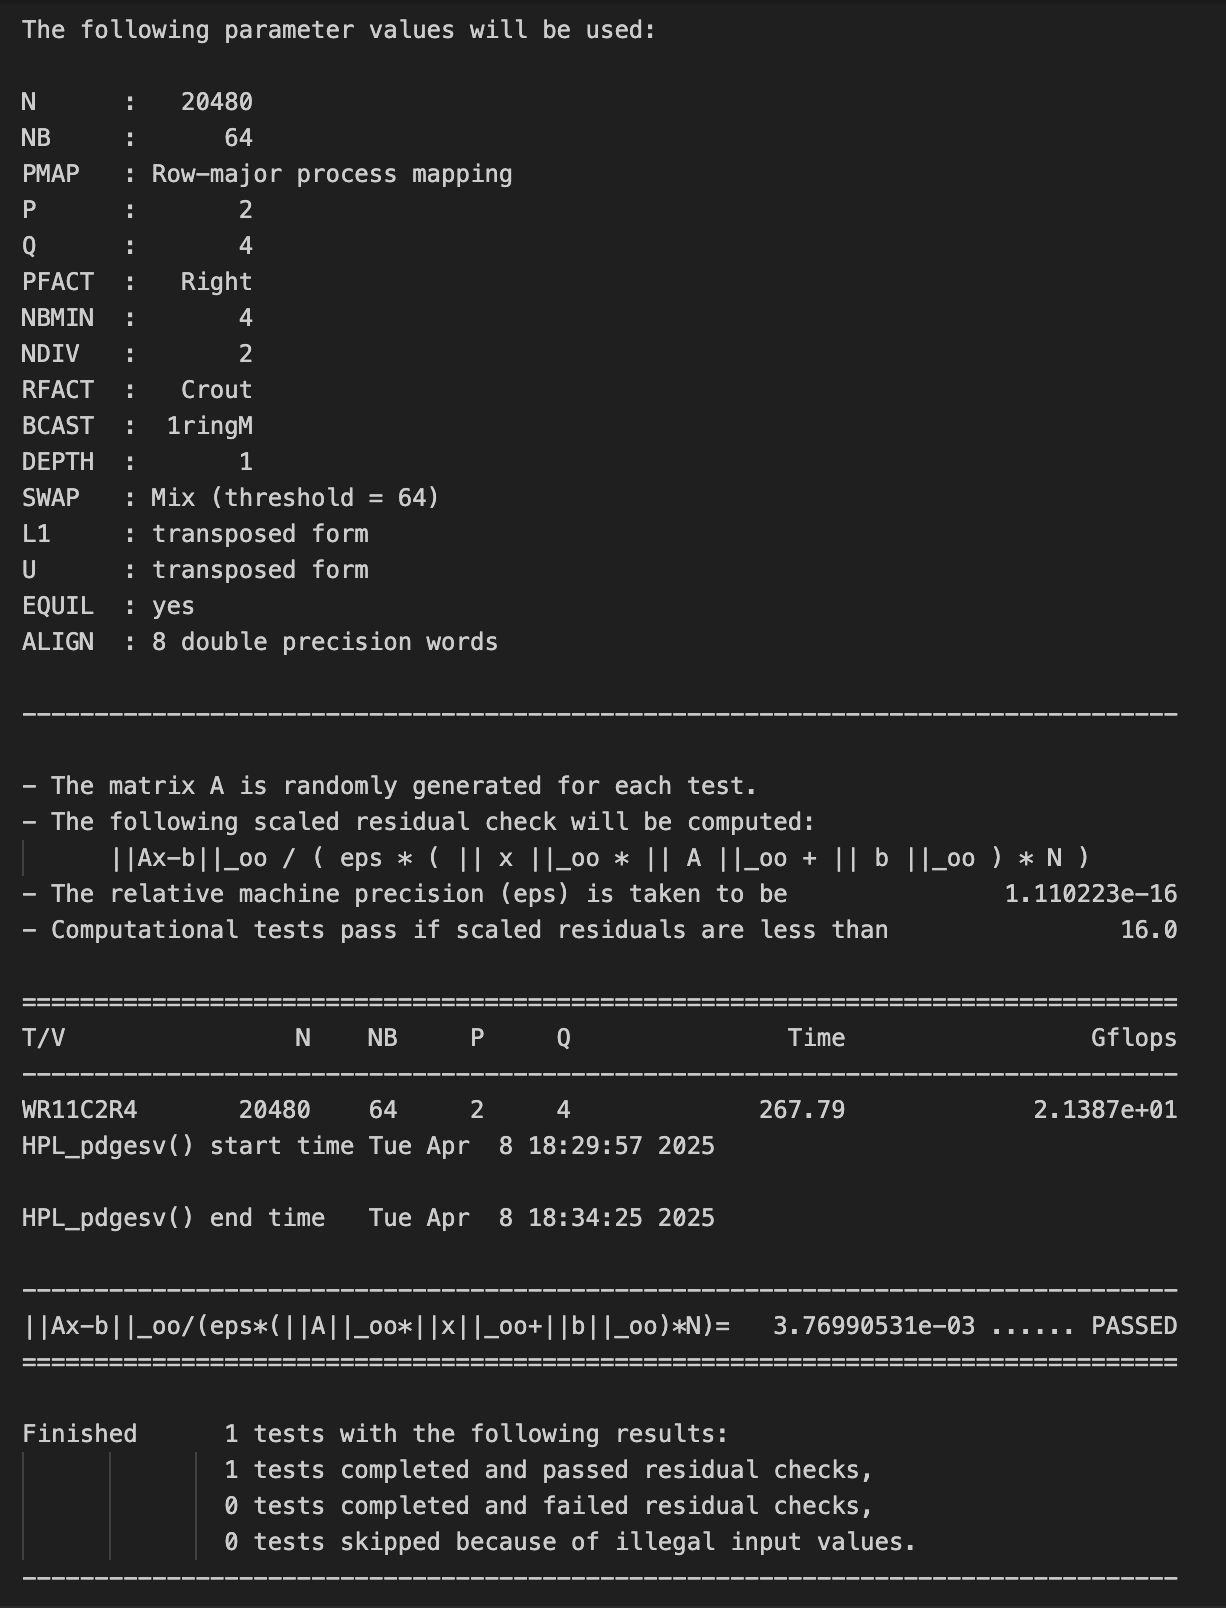
\includegraphics[width=0.8\textwidth]{./img/HPL.png}
\end{figure}

The image shows PASSED and Gflops is 2.1387e+01. Gflops means the performance of the matrix multiplication. The higher the Gflops, the better the performance.

\clearpage

\subsection*{Results under different parameters}

The following image shows the results under different parameters.

\subsubsection*{(N, NB, P, Q) = (1000, 64, 2, 2)}

It is run with the following command:

\begin{lstlisting}[language=bash, basicstyle=\ttfamily\small, numbers=left, numberstyle=\tiny\color{gray}, stepnumber=1, frame=single]
$ mpirun -np 4 ./xhpl
\end{lstlisting}

The following image shows the results.

\begin{figure}[htbp]
    \centering
    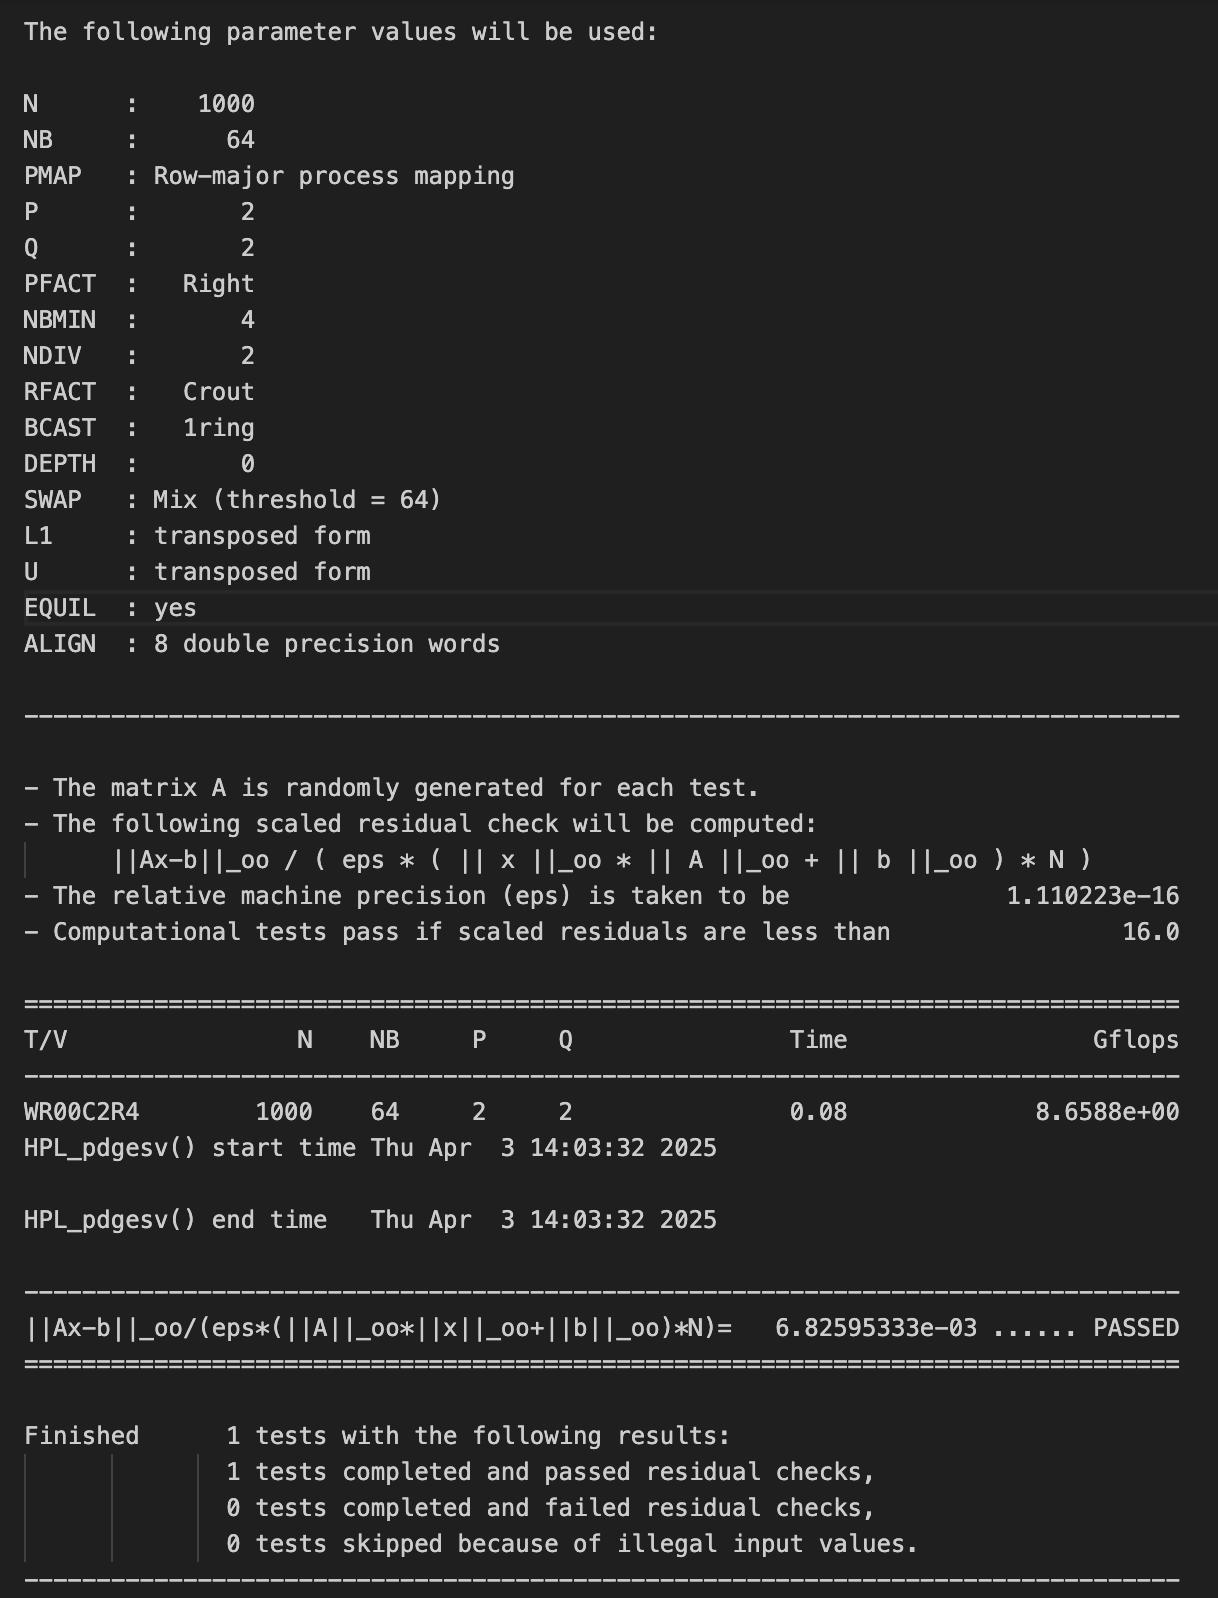
\includegraphics[width=0.8\textwidth]{./img/HPL_1000_64_2_2.png}
\end{figure}

The image shows PASSED and Gflops is 8.6588e+00.

\clearpage

\subsubsection*{(N, NB, P, Q) = (5000, 128, 4, 2)}

It is run with the following command:

\begin{lstlisting}[language=bash, basicstyle=\ttfamily\small, numbers=left, numberstyle=\tiny\color{gray}, stepnumber=1, frame=single]
$ mpirun -np 8 ./xhpl
\end{lstlisting}

The following image shows the results.

\begin{figure}[htbp]
    \centering
    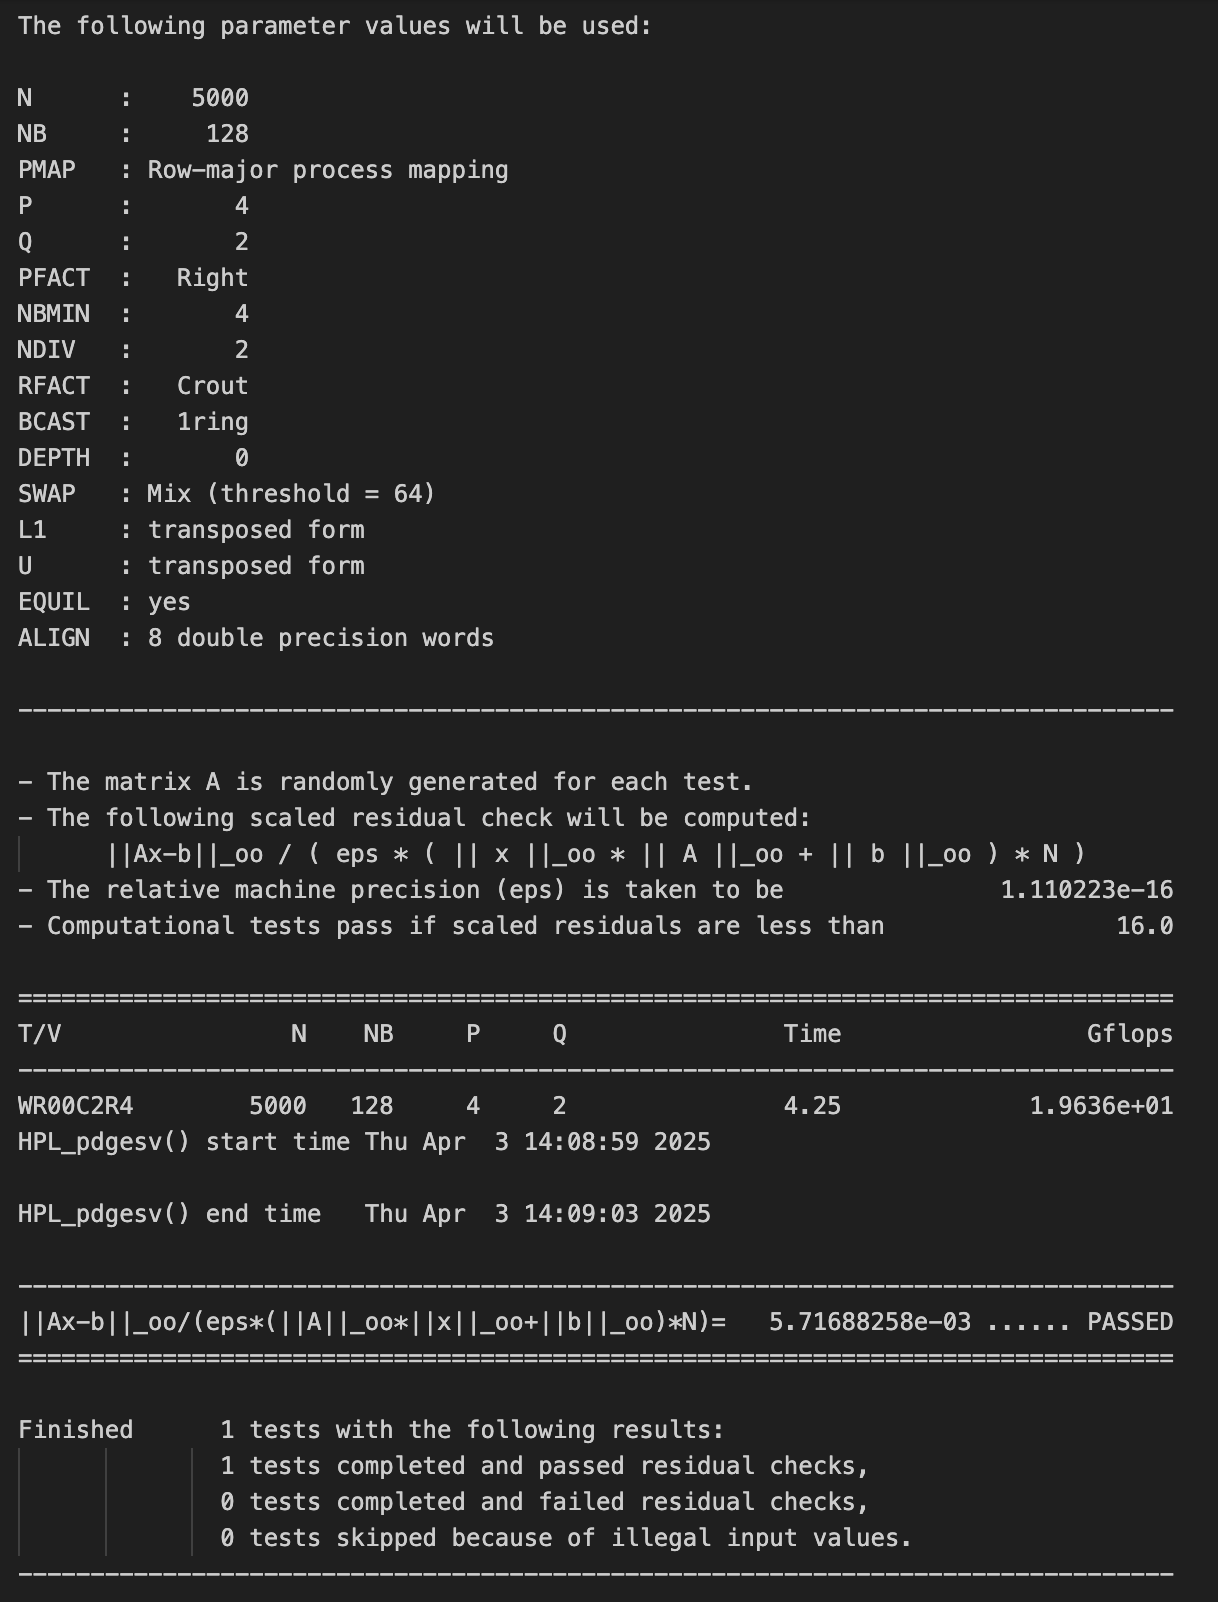
\includegraphics[width=0.8\textwidth]{./img/HPL_5000_128_4_2.png}
\end{figure}

The image shows PASSED and Gflops is 1.9636e+01.

\clearpage

\subsubsection*{(N, NB, P, Q) = (12000, 256, 2, 4)}

It is run with the following command:

\begin{lstlisting}[language=bash, basicstyle=\ttfamily\small, numbers=left, numberstyle=\tiny\color{gray}, stepnumber=1, frame=single]
$ mpirun -np 8 ./xhpl
\end{lstlisting}

The following image shows the results.

\begin{figure}[htbp]
    \centering
    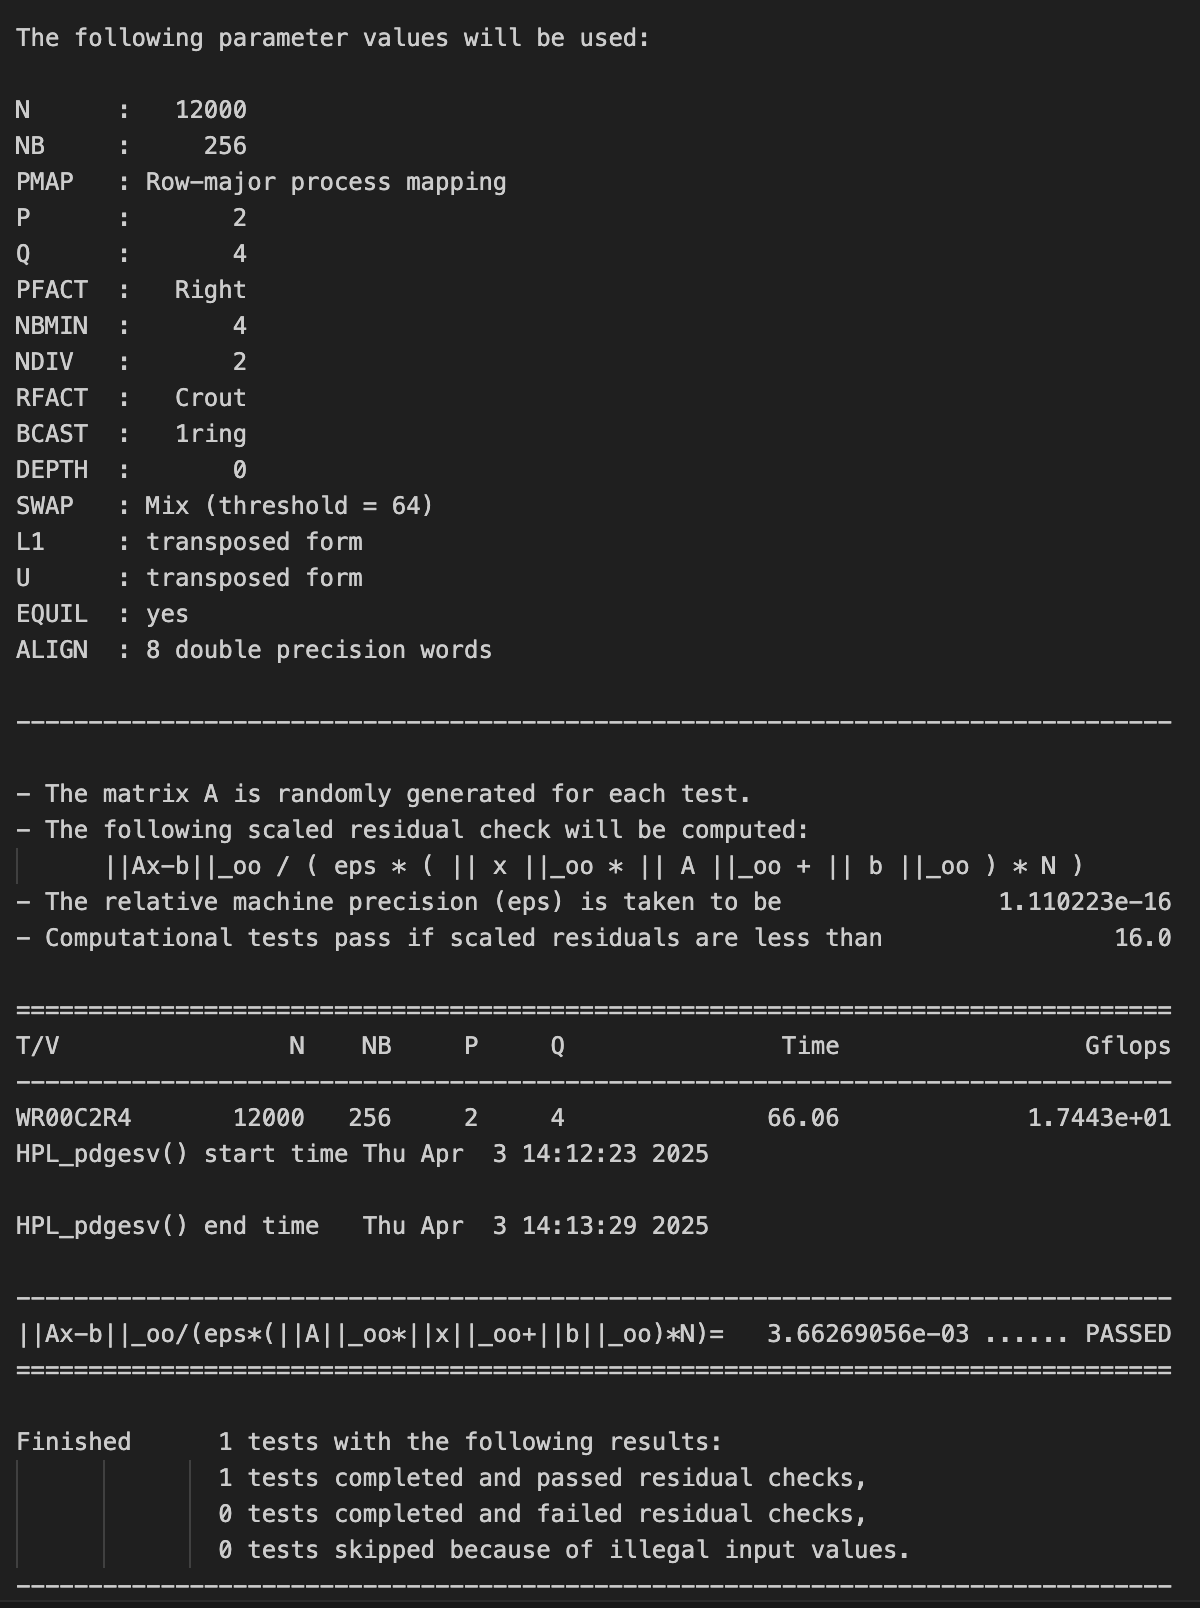
\includegraphics[width=0.8\textwidth]{./img/HPL_12000_256_2_4.png}
\end{figure}

The image shows PASSED and Gflops is 1.7433e+01.

\clearpage

\section*{HPCG (High Performance Conjugate Gradient)}
\subsection*{Setting of nx, ny, nz}

% The parameters nx, ny, and nz define the dimensions of the 3D matrix used in HPCG. The matrix has dimensions $nx \times ny \times nz$ with a total of $nx \times ny \times nz$ elements.

% \vspace{1em}

% Using our previously determined total memory of \texttt{3930592 kB}, we can convert this to bytes:
% \begin{align*}
%     \texttt{Total\ Memory} &= 3930592 \times 1024 \text{ bytes} \\
%     &= 4026531840 \text{ bytes}
% \end{align*}

% To avoid OOM (Out Of Memory) errors, we allocate 80\% of the total memory:
% \begin{align*}
%     \texttt{Available\ Memory} &= 4026531840 \times 0.8 \text{ bytes} \\
%     &= 3221225472 \text{ bytes}
% \end{align*}

% Assuming each grid point requires 120 bytes, we can calculate the total number of grid points:
% \begin{align*}
%     \texttt{Total\ Grid\ Points} &= \frac{\texttt{Available\ Memory}}{120 \text{ bytes}} \\
%     &= \frac{3221225472}{120} \\
%     &\approx 26843545
% \end{align*}

% For a balanced 3D grid where $nx \times ny \times nz = 26843545$, we can set all dimensions equal:
% \begin{align*}
%     nx = ny = nz &= \sqrt[3]{26843545} \\
%     &\approx 299
% \end{align*}

% Since HPCG performs optimally when dimensions are multiples of 8, we round up to $nx = ny = nz = 304$.

The parameters nx, ny, and nz define the dimensions of the 3D matrix used in HPCG. The matrix has dimensions $nx \times ny \times nz$ with a total of $nx \times ny \times nz$ elements.

\vspace{1em}

I set nx, ny, and nz to 96. and use the following command to run HPCG:

\begin{lstlisting}[language=bash, basicstyle=\ttfamily\small, numbers=left, numberstyle=\tiny\color{gray}, stepnumber=1, frame=single]
$ mpirun -np 8 ./xhpcg
\end{lstlisting}

This value was determined through testing to be the maximum that avoids OOM errors.

\subsection*{Setting of Time}

In HPCG, the time parameter specifies the maximum duration (in seconds) allocated for the benchmark run.

\vspace{1em}

I set the time to 10 seconds. Because the time is too long, it will take a long time to run.

\subsection*{Results}

\begin{figure}[htbp]
    \centering
    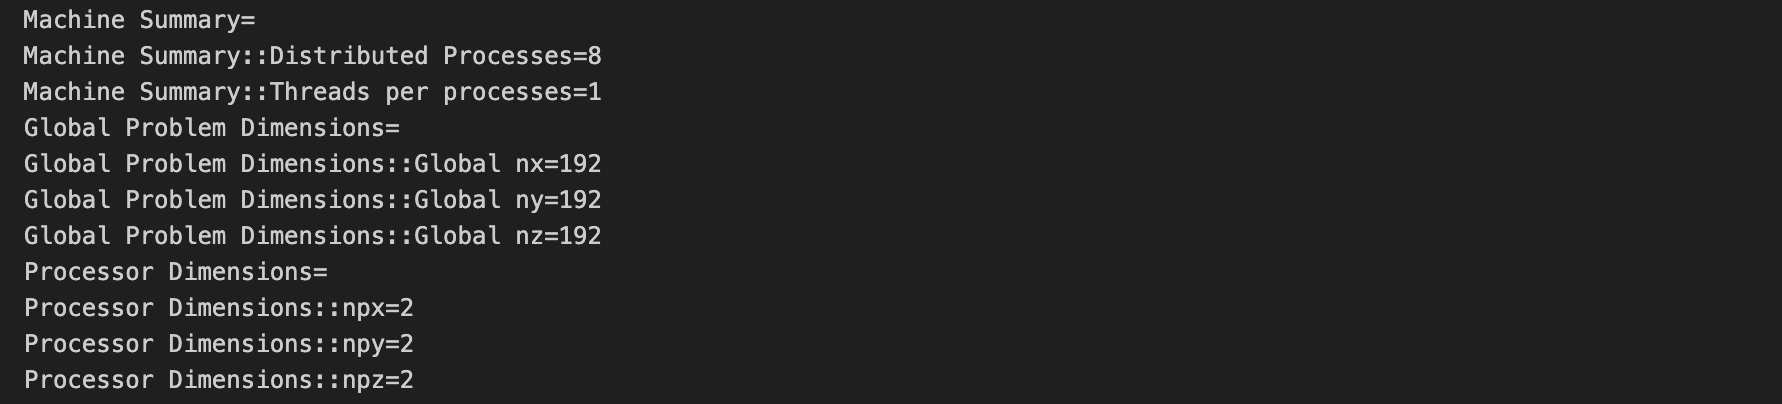
\includegraphics[width=0.8\textwidth]{./img/HPCG_Machine.png}
\end{figure}

The image shows that it is actually decomposed into a $2 \times 2 \times 2$ grid across three dimensions. In effect, the matrix being processed is $(96 \times 2) \times (96 \times 2) \times (96 \times 2)$.

\begin{figure}[htbp]
    \centering
    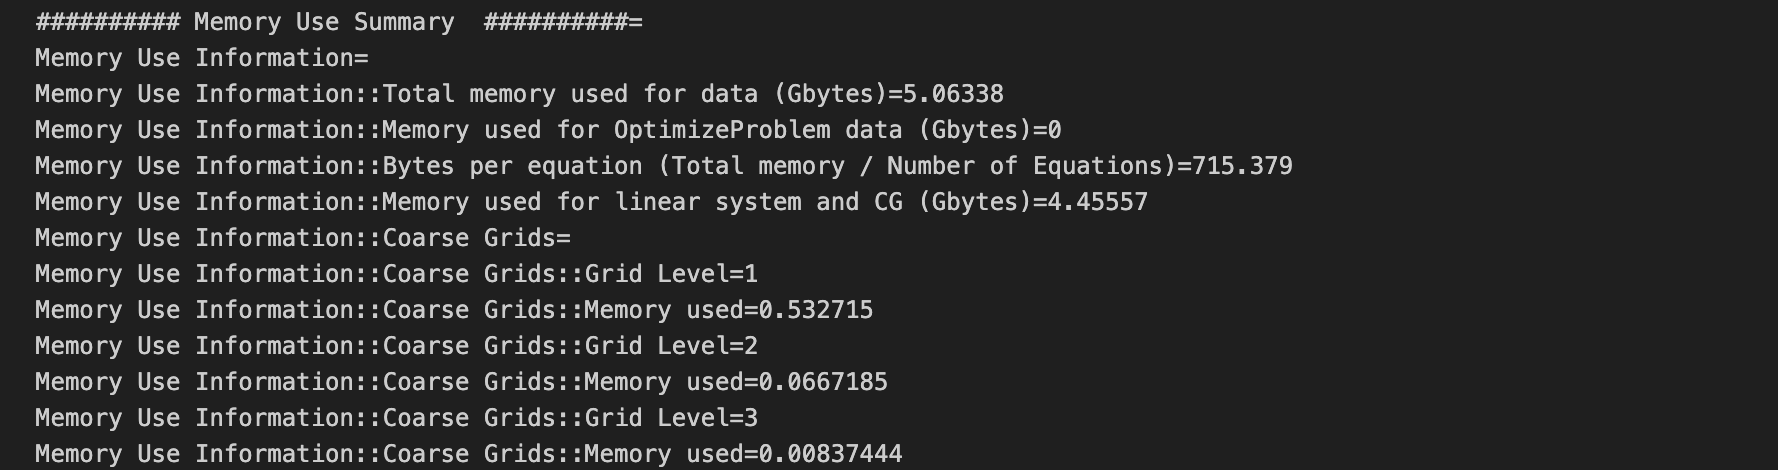
\includegraphics[width=0.8\textwidth]{./img/HPCG_Memory.png}
\end{figure}

The memory usage is reported as 5.06338 GB. Although this exceeds the memory size, it is likely that swap space or system memory management is compensating.

\clearpage

\begin{figure}[htbp]
    \centering
    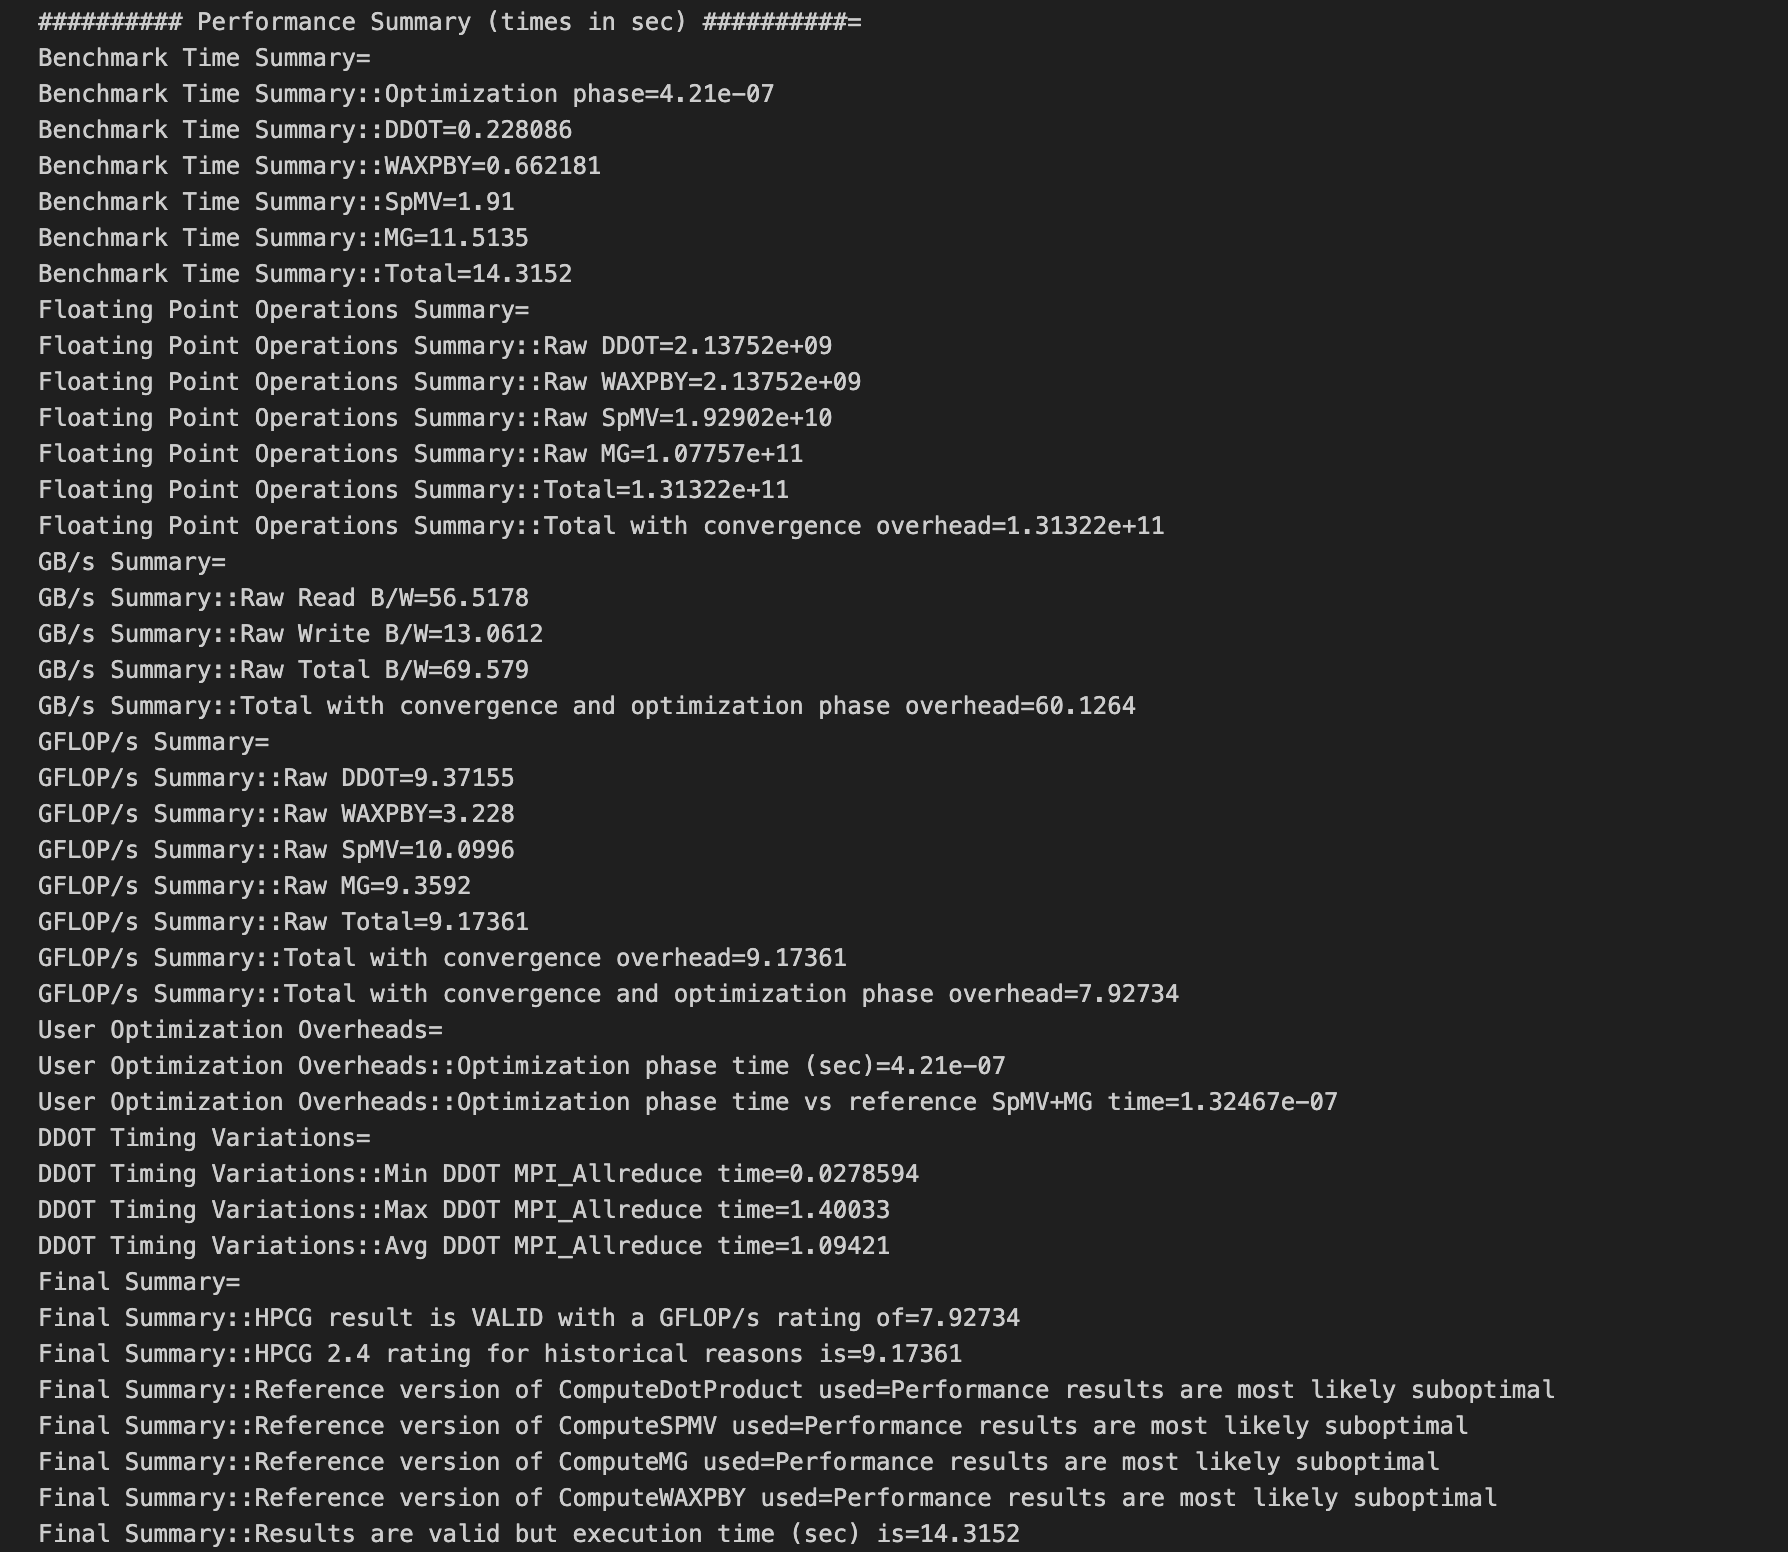
\includegraphics[width=0.8\textwidth]{./img/HPCG_Performance.png}
\end{figure}

The image shows HPCG result is VALID with a GFLOP/s rating of=7.92734.

\clearpage

\subsection*{Results under different parameters}

\subsubsection*{(nx, ny, nz) = (56, 56, 56)}

It is run with the following command:

\begin{lstlisting}[language=bash, basicstyle=\ttfamily\small, numbers=left, numberstyle=\tiny\color{gray}, stepnumber=1, frame=single]
$ mpirun -np 8 ./xhpcg
\end{lstlisting}

\begin{figure}[htbp]
    \centering
    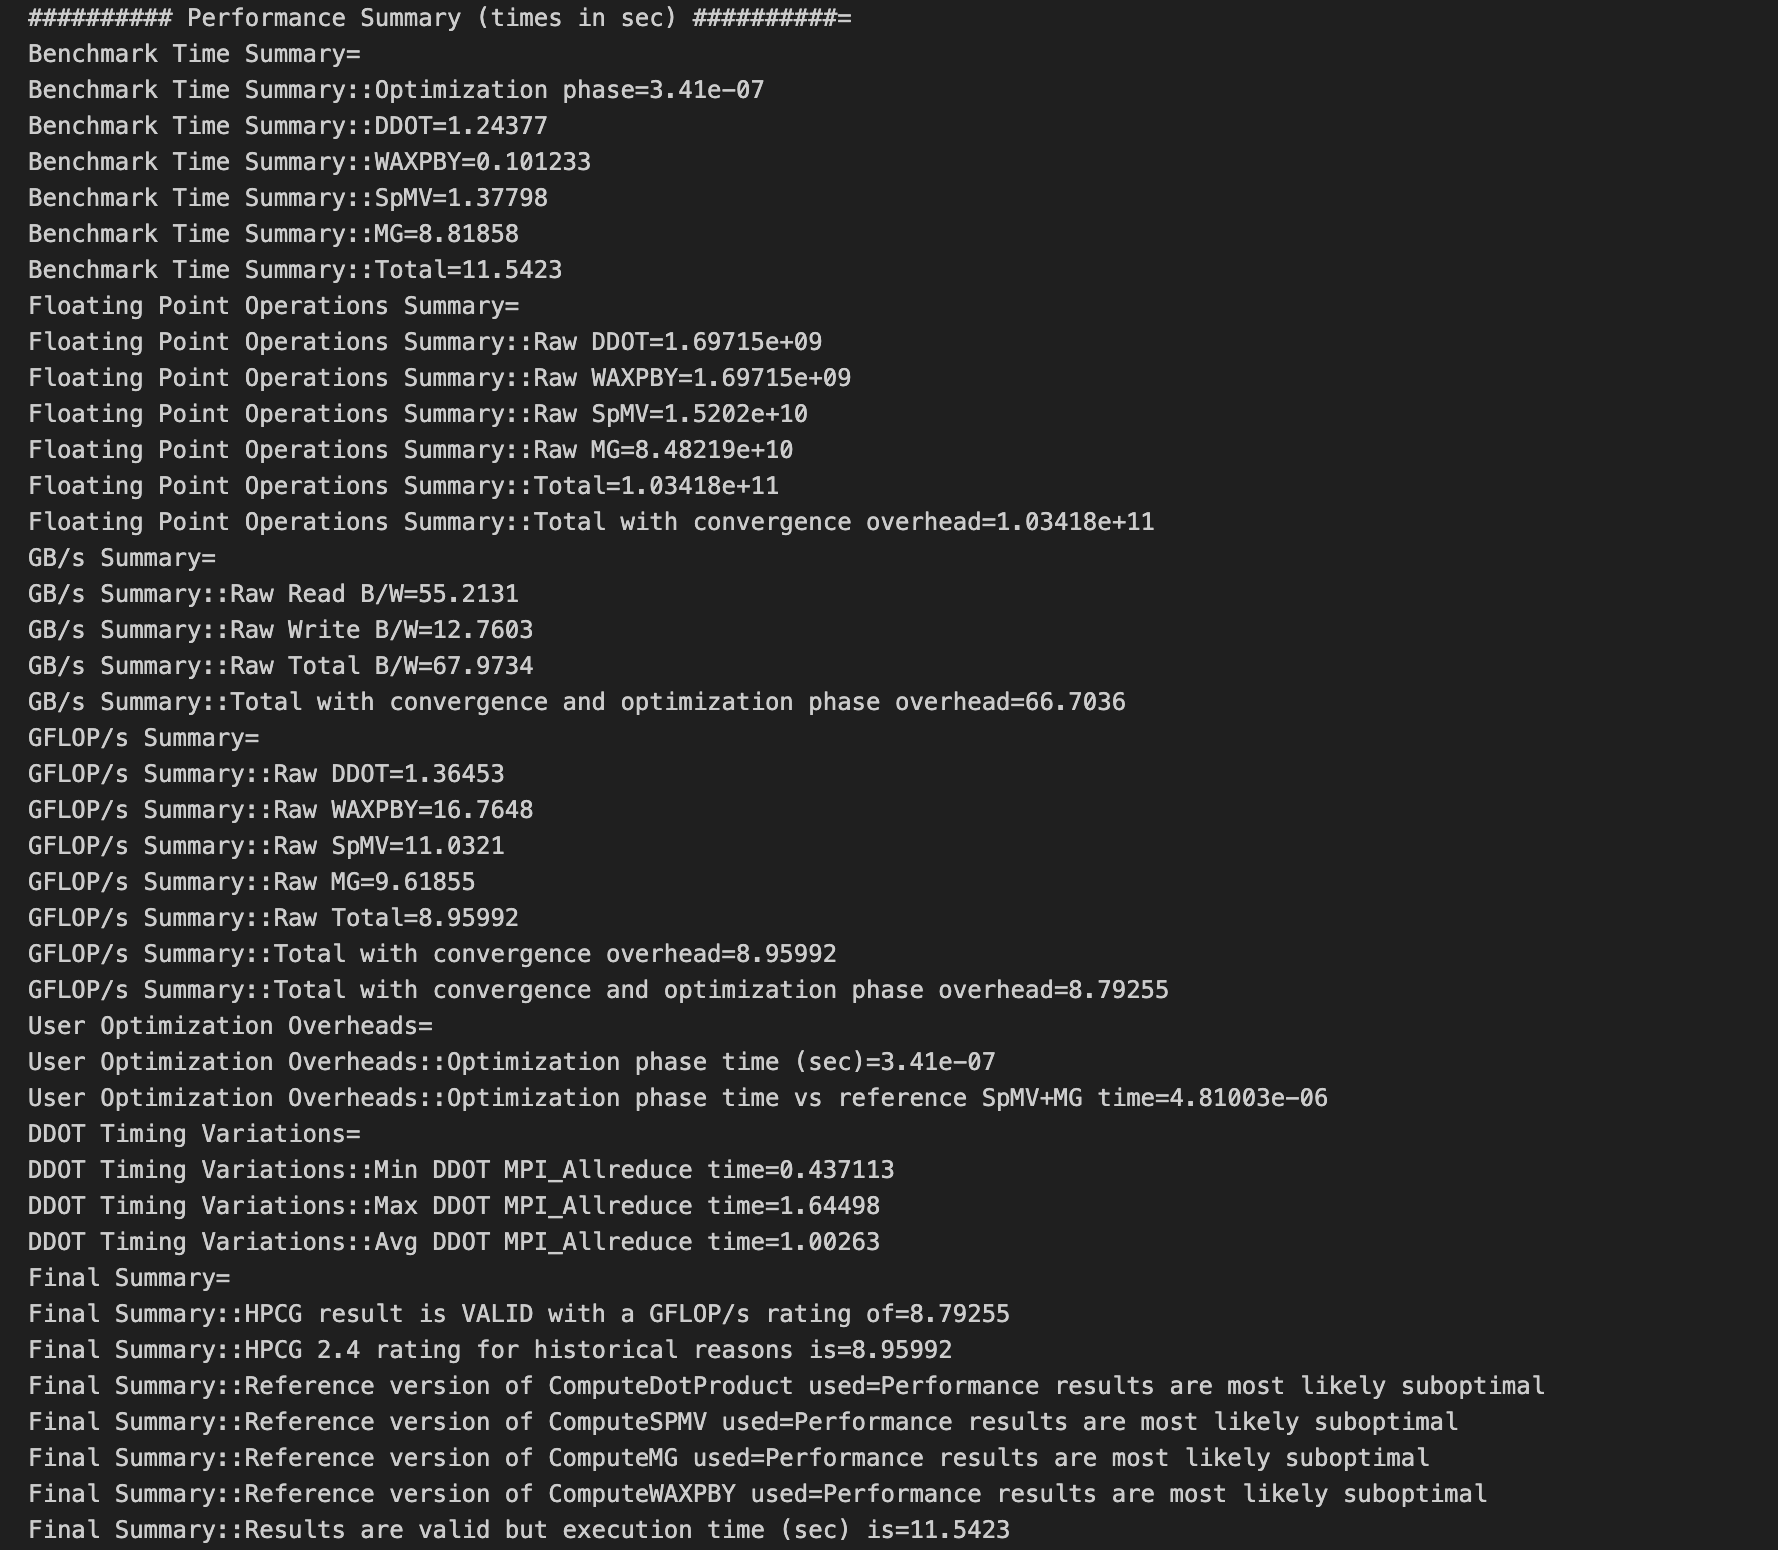
\includegraphics[width=0.8\textwidth]{./img/HPCG_56_56_56.png}
\end{figure}

The image shows HPCG result is VALID with a GFLOP/s rating of=8.79255.

\clearpage

\subsubsection*{(nx, ny, nz) = (64, 64, 64)}

It is run with the following command:

\begin{lstlisting}[language=bash, basicstyle=\ttfamily\small, numbers=left, numberstyle=\tiny\color{gray}, stepnumber=1, frame=single]
$ mpirun -np 8 ./xhpcg
\end{lstlisting}

\begin{figure}[htbp]
    \centering
    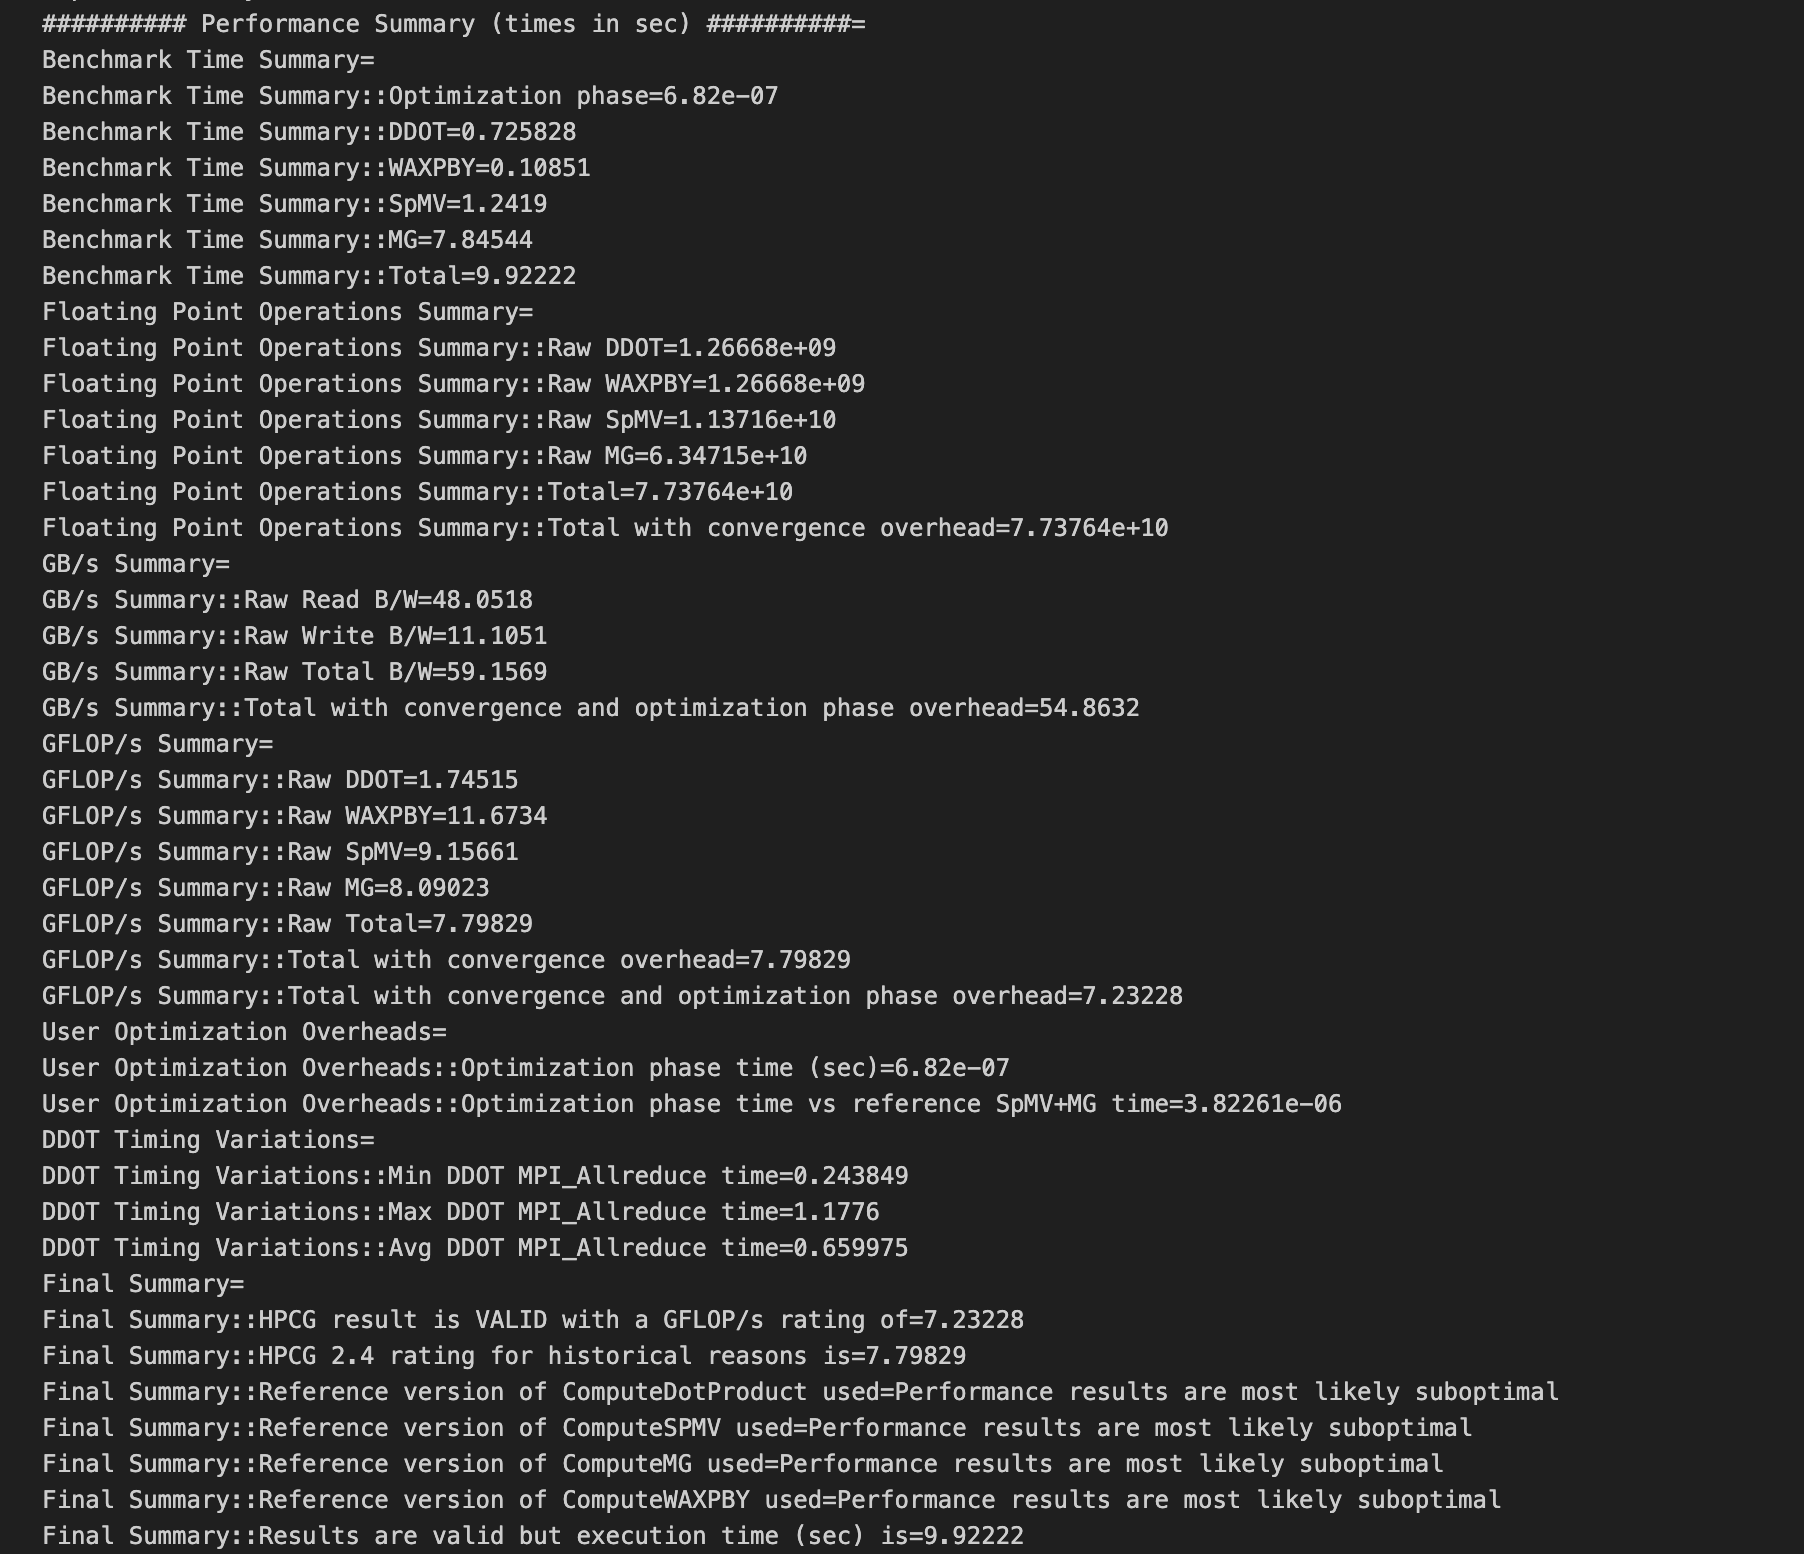
\includegraphics[width=0.8\textwidth]{./img/HPCG_64_64_64.png}
\end{figure}

The image shows HPCG result is VALID with a GFLOP/s rating of=7.23228.

\end{document}
